\documentclass[11pt,a4paper]{article}

\usepackage[margin=22mm,headheight=15pt]{geometry}
\usepackage[T1]{fontenc}
\usepackage[utf8]{inputenc}
\usepackage{newtxtext,newtxmath}
\usepackage{microtype}
\usepackage{amsmath,mathtools,bm}
\usepackage{graphicx}
\usepackage{booktabs,tabularx,longtable,array,multirow}
\usepackage{caption,subcaption}
\usepackage{enumitem}
\usepackage{float}
\usepackage{placeins}
\usepackage{xcolor}
\usepackage[most]{tcolorbox}
\usepackage{titlesec}
\usepackage{fancyhdr}
\usepackage{hyperref}
\usepackage[nameinlink,capitalise,noabbrev]{cleveref}
\usepackage{listings}
\usepackage{setspace}
\usepackage{appendix}
\usepackage{multicol}

\graphicspath{{figures/}}

\definecolor{navy}{HTML}{1F4E79}
\definecolor{brick}{HTML}{B03A2E}
\definecolor{teal}{HTML}{2A7F62}
\definecolor{gold}{HTML}{B58900}
\definecolor{purple}{HTML}{6C5B7B}
\definecolor{softblue}{HTML}{EDF4F8}
\definecolor{softred}{HTML}{FBF0ED}
\definecolor{softgreen}{HTML}{EDF7F2}
\definecolor{softgold}{HTML}{FFF8E8}
\definecolor{softgray}{HTML}{F3F4F5}
\definecolor{ink}{HTML}{202124}

\hypersetup{
  colorlinks=true,
  linkcolor=navy,
  citecolor=teal,
  urlcolor=purple,
  pdftitle={Experiment 1: Joint Score Dynamics on a Rotating Ring},
  pdfauthor={Giovanni Mantovani}
}

\titleformat{\section}{\Large\bfseries\color{navy}}{\thesection}{0.7em}{}
\titleformat{\subsection}{\large\bfseries\color{ink}}{\thesubsection}{0.65em}{}
\titleformat{\subsubsection}{\normalsize\bfseries\color{teal}}{\thesubsubsection}{0.6em}{}
\titlespacing*{\section}{0pt}{2.4ex plus 0.8ex minus 0.3ex}{1.1ex}
\titlespacing*{\subsection}{0pt}{2.0ex plus 0.6ex minus 0.2ex}{0.8ex}

\pagestyle{fancy}
\fancyhf{}
\fancyhead[L]{\small Experiment 1: rotating ring}
\fancyhead[R]{\small Joint score dynamics}
\fancyfoot[C]{\thepage}
\renewcommand{\headrulewidth}{0.3pt}

\newcommand{\R}{\mathbb{R}}
\newcommand{\E}{\mathbb{E}}
\newcommand{\N}{\mathcal{N}}
\newcommand{\given}{\,\vert\,}
\newcommand{\score}{\bm S}
\newcommand{\margscore}{\bm s^{\mathrm{marg}}}
\newcommand{\mt}{m_t}
\newcommand{\Dt}{\Delta_t}
\newcommand{\Cov}{\operatorname{Cov}}
\newcommand{\Var}{\operatorname{Var}}
\newcommand{\diag}{\operatorname{diag}}
\newcommand{\tr}{\operatorname{tr}}
\newcommand{\Id}{I}
\newcommand{\dd}{\,\mathrm d}
\newcommand{\e}{\mathrm e}
\newcommand{\wrap}{\operatorname{wrap}}
\newcommand{\WN}{\operatorname{WN}}
\newcommand{\RMSE}{\operatorname{RMSE}}

\newtcolorbox{keyresult}[1][] {
  enhanced, breakable,
  colback=softblue, colframe=navy,
  boxrule=0.75pt, arc=1.5mm,
  left=2mm,right=2mm,top=1.5mm,bottom=1.5mm,
  title={#1}, colbacktitle=navy, coltitle=white, fonttitle=\bfseries
}
\newtcolorbox{intuition}[1][] {
  enhanced, breakable,
  colback=softgreen, colframe=teal,
  boxrule=0.7pt, arc=1.5mm,
  left=2mm,right=2mm,top=1.5mm,bottom=1.5mm,
  title={#1}, colbacktitle=teal, coltitle=white, fonttitle=\bfseries
}
\newtcolorbox{caution}[1][] {
  enhanced, breakable,
  colback=softred, colframe=brick,
  boxrule=0.7pt, arc=1.5mm,
  left=2mm,right=2mm,top=1.5mm,bottom=1.5mm,
  title={#1}, colbacktitle=brick, coltitle=white, fonttitle=\bfseries
}
\newtcolorbox{definitionbox}[1][] {
  enhanced, breakable,
  colback=softgold, colframe=gold,
  boxrule=0.7pt, arc=1.5mm,
  left=2mm,right=2mm,top=1.5mm,bottom=1.5mm,
  title={#1}, colbacktitle=gold, coltitle=black!78, fonttitle=\bfseries
}
\newtcolorbox{derivation}[1][] {
  enhanced, breakable,
  colback=softgray, colframe=black!35,
  boxrule=0.55pt, arc=1.2mm,
  left=2mm,right=2mm,top=1.2mm,bottom=1.2mm,
  title={#1}, colbacktitle=black!45, coltitle=white, fonttitle=\bfseries
}

\captionsetup{font=small,labelfont=bf,labelsep=period}
\setlist[itemize]{leftmargin=1.6em,itemsep=0.25em,topsep=0.35em}
\setlist[enumerate]{leftmargin=1.8em,itemsep=0.3em,topsep=0.35em}
\setlength{\parindent}{0pt}
\setlength{\parskip}{0.55em}
\allowdisplaybreaks
\onehalfspacing

\lstset{
  basicstyle=\ttfamily\small,
  backgroundcolor=\color{softgray},
  frame=single,
  rulecolor=\color{black!20},
  breaklines=true,
  columns=fullflexible,
  showstringspaces=false
}

\begin{document}
\hypersetup{pageanchor=false}

\begin{titlepage}
\thispagestyle{empty}
\vspace*{5mm}
{\Large\color{navy}\bfseries Master's thesis research note}\par
\vspace{6mm}
{\fontsize{29}{33}\selectfont\bfseries Experiment 1: Joint Score Dynamics on a Rotating Ring}\par
\vspace{3mm}
{\Large From an exactly solvable surrogate to the board-faithful polar process}\par
\vspace{7mm}
\begin{center}
\includegraphics[width=0.98\textwidth]{fig01_model_overview.pdf}
\end{center}
\vfill
{\large Giovanni Mantovani}\par
{\normalsize Bocconi University -- Data Science and Business Analytics}\par
{\normalsize 25 July 2026}\par
\vspace{4mm}
{\small This document consolidates the first rotating-circle experiment discussed on the board with Marc M\'ezard. It reconstructs every model and identity from first principles, distinguishes the original polar process from its exactly solvable surrogate, and documents all simulations, diagnostics, numerical checks, and limitations.}\par
\end{titlepage}

\hypersetup{pageanchor=true}
\pagenumbering{roman}

\begin{abstract}
A dynamic object is a whole trajectory, not a set of independent frames. We study the joint diffusion score of a noisy rotating trajectory near a unit ring. The note proceeds in two stages. First, a Cartesian rotating-random-walk surrogate is solved exactly: a known rotation can be removed by an orthogonal change of coordinates, after which the noised score reduces to a Gaussian random-walk term plus a low-dimensional correction generated by the shared ring anchor. Second, the original polar model is treated directly. Its exact radial and angular transition laws are derived from the stochastic differential equations, its noised score is written as a posterior smoothing mean, and its response to perturbing another frame is shown to equal a posterior covariance through a static fluctuation-response identity. A first-order Taylor expansion gives an interpretable linear-Gaussian approximation. Numerical experiments then measure three distinct quantities: the absolute intensity of cross-frame influence, its temporal range, and the finite receptive field needed to approximate the full joint score. The central finding is robust in both models: increasing diffusion time broadens the normalized temporal range of the remaining dependence while strongly reducing its absolute intensity. In the original polar process, tangential information propagates farther than radial information at low noise because radial fluctuations are mean-reverting whereas the angular phase is highly coherent.
\end{abstract}

\begin{keyresult}[Main answers]
\begin{enumerate}
\item The clean trajectory is Markovian and its clean score is local, but the score of the \emph{noised joint trajectory} is generally nonlocal.
\item Clean Markovity is still highly useful: all distant influence must be transmitted through repeated one-step transitions, so nonlocality has a structured temporal profile rather than an arbitrary one.
\item The cross-frame Jacobian is exactly controlled by posterior covariance:
\[
\frac{\partial S_k}{\partial x_j}
=-\frac{\delta_{kj}}{\Delta_t}I_2
+\frac{m_t^2}{\Delta_t^2}\Cov(A_k,A_j\mid X_t=x).
\]
\item Response \emph{range}, response \emph{intensity}, and functional \emph{receptive field} are different observables and can move in different directions.
\item At low diffusion noise, tangential information travels much farther than radial information. At large diffusion noise, both channels are broad but weak and the score approaches $-x$.
\item A local Taylor model reproduces the score accurately near one inferred rotating branch, but it cannot represent global angular wrapping or multimodal phase uncertainty.
\end{enumerate}
\end{keyresult}

\setcounter{tocdepth}{2}
\tableofcontents
\clearpage
\pagenumbering{arabic}

% ============================================================================
\section{Problem statement and notation}
% ============================================================================

\subsection{The object of study}

We observe a planar trajectory at internal times
\[
 u_k=kh,\qquad k=0,1,\ldots,T-1.
\]
The clean frame is $A_k\in\R^2$, and the complete datum is the stacked vector
\begin{equation}
 A=(A_0,A_1,\ldots,A_{T-1})\in\R^{2T}.
 \label{eq:whole-trajectory}
\end{equation}
One data point is therefore one trajectory. The $T$ frames are correlated coordinates of that data point.

A second clock, diffusion time $t\ge 0$, controls how strongly the whole vector is corrupted. The two clocks have different roles:
\begin{itemize}
\item internal time $u_k$ describes the clean physical dynamics;
\item diffusion time $t$ describes the artificial noising channel used by the generative model.
\end{itemize}

\begin{figure}[H]
\centering
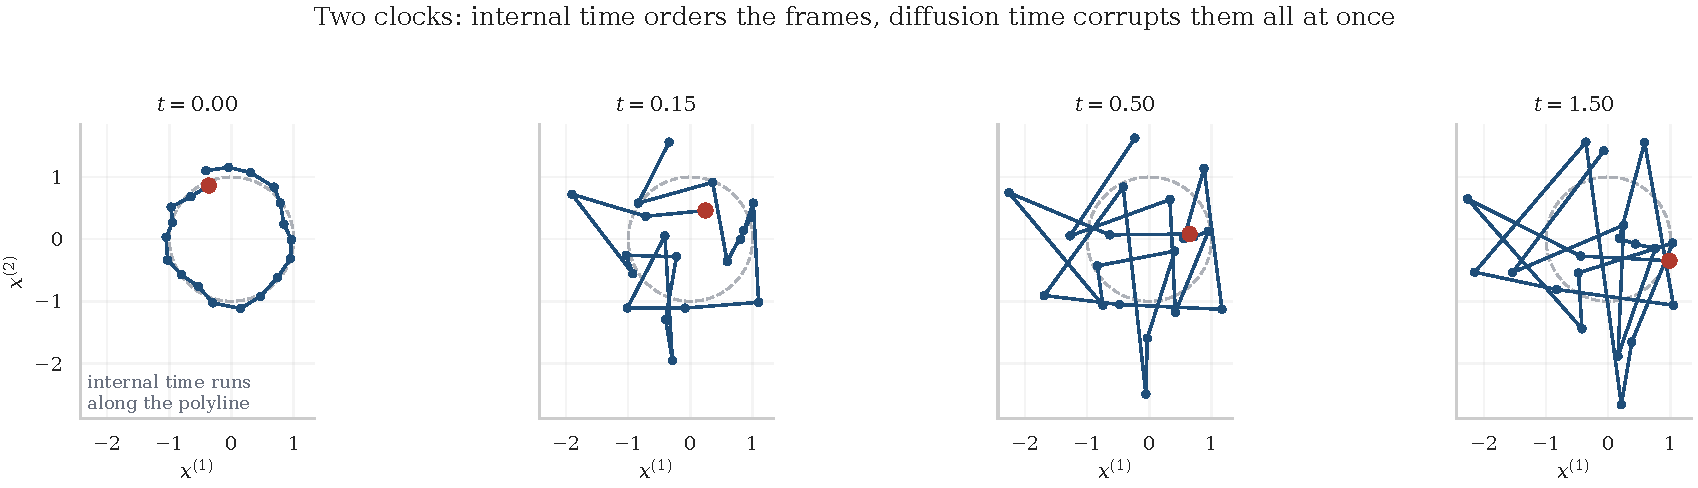
\includegraphics[width=\textwidth]{fig02_two_clocks.pdf}
\caption{The two clocks. Internal time is the ordering of points along the polyline. Diffusion time $t$ shrinks and corrupts every frame simultaneously. The same standardized noise realization is used in all panels to isolate the effect of $t$.}
\label{fig:two-clocks}
\end{figure}

\subsection{Research question}

The broad question is:
\begin{keyresult}[Research question]
How can the Markov structure of the clean rotating trajectory be exploited to compute and understand the dynamics of the joint diffusion score?
\end{keyresult}

We make this operational through four subquestions.
\begin{enumerate}
\item How different is the joint score from a collection of one-frame marginal scores?
\item How strongly does observed frame $j$ influence the score acting on frame $k$?
\item How does that influence decay with temporal lag $|j-k|$?
\item How many nearby frames are needed to approximate the full score to a prescribed accuracy?
\end{enumerate}

\subsection{Notation table}

\begin{table}[H]
\centering
\small
\begin{tabularx}{\textwidth}{@{}lX@{}}
\toprule
Symbol & Meaning \\
\midrule
$k,j$ & discrete internal-time indices \\
$h$ & spacing between consecutive clean frames \\
$t$ & diffusion time \\
$A_k$ & clean Cartesian frame \\
$X_k$ & noised Cartesian frame at diffusion time $t$ \\
$R_k,\Theta_k$ & latent radius and angle in the original polar model \\
$m_t=e^{-t}$ & signal attenuation of the variance-preserving OU channel \\
$\Delta_t=1-e^{-2t}$ & variance added by the OU channel \\
$S_k(x,t)$ & $k$th two-dimensional block of the joint score \\
$J_{kj}(x,t)$ & block response $\partial S_k/\partial x_j\in\R^{2\times2}$ \\
$L$ & radius of a temporal observation window around frame $k$ \\
\bottomrule
\end{tabularx}
\end{table}

% ============================================================================
\section{The common diffusion identities}
% ============================================================================

The surrogate and the original polar process have different clean dynamics, but the same noising channel. It is useful to derive the diffusion identities once.

\subsection{Solving the variance-preserving Ornstein--Uhlenbeck channel}

The forward noising process in diffusion time is
\begin{equation}
 \dd X_t=-X_t\,\dd t+\sqrt{2}\,\dd W_t,
 \qquad X_0=A,
 \label{eq:ou-sde}
\end{equation}
where $W_t$ is Brownian motion in $\R^{2T}$. Multiply by the integrating factor $\e^t$:
\[
 \dd(\e^tX_t)=\sqrt{2}\,\e^t\dd W_t.
\]
Integrating from $0$ to $t$ gives
\[
 \e^tX_t-A=\sqrt{2}\int_0^t\e^s\dd W_s,
\]
so
\begin{equation}
 X_t=\e^{-t}A+\sqrt{2}\int_0^t\e^{-(t-s)}\dd W_s.
 \label{eq:ou-integrated}
\end{equation}
The stochastic integral is Gaussian with covariance
\[
 2\int_0^t\e^{-2(t-s)}\dd s
 =1-\e^{-2t}.
\]
Therefore
\begin{keyresult}[Exact OU channel]
\begin{equation}
 \boxed{
 X_t=m_tA+\sqrt{\Delta_t}\,Z,
 \qquad m_t=\e^{-t},\qquad \Delta_t=1-\e^{-2t},
 \qquad Z\sim\N(0,I_{2T}).}
 \label{eq:ou-channel}
\end{equation}
\end{keyresult}
This is the standard variance-preserving OU channel used in the diffusion notes of M\'ezard and in the statistical-physics analyses of diffusion models \cite{mezardnotes,biroli2023,biroli2024}.

\subsection{The joint score as a posterior denoiser}

The noised joint density is
\begin{equation}
 p_t(x)=\int p_0(a)\,\N(x;m_ta,\Delta_t I_{2T})\,\dd a.
 \label{eq:noised-density}
\end{equation}
Differentiate under the integral:
\begin{align}
 \nabla_x p_t(x)
 &=\int p_0(a)\,\N(x;m_ta,\Delta_t I)
 \frac{m_ta-x}{\Delta_t}\,\dd a.
\end{align}
Dividing by $p_t(x)$ converts the normalized integrand into the posterior $p(a\mid x)$:
\begin{keyresult}[Score--posterior identity]
\begin{equation}
 \boxed{
 \score(x,t)=\nabla_x\log p_t(x)
 =\frac{m_t\E[A\mid X_t=x]-x}{\Delta_t}.}
 \label{eq:score-posterior}
\end{equation}
\end{keyresult}
For one frame,
\begin{equation}
 \boxed{
 S_k(x,t)=\frac{m_t\E[A_k\mid X_0=x_0,\ldots,X_{T-1}=x_{T-1}]-x_k}{\Delta_t}.}
 \label{eq:block-score}
\end{equation}
The score at frame $k$ is therefore a \emph{smoothing} estimate: it uses all observations, past and future, to estimate one clean frame.

\subsection{Why the marginal score is a different object}

The one-frame marginal score is
\begin{equation}
 s_k^{\rm marg}(x_k,t)
 =\frac{m_t\E[A_k\mid X_k=x_k]-x_k}{\Delta_t}.
\end{equation}
Subtracting it from the joint score gives
\begin{equation}
 \boxed{
 S_k(x,t)-s_k^{\rm marg}(x_k,t)
 =\frac{m_t}{\Delta_t}
 \left(
 \E[A_k\mid X_{0:T-1}=x]-\E[A_k\mid X_k=x_k]
 \right).}
 \label{eq:joint-marg-gap}
\end{equation}
The difference is exactly the extra denoising information supplied by the rest of the trajectory.

\subsection{A static fluctuation--response identity}

Expand the Gaussian channel inside the posterior:
\begin{align}
 p(a\mid x)
 &\propto p_0(a)
 \exp\left[-\frac{\|x-m_ta\|^2}{2\Delta_t}\right]\\
 &\propto p_0(a)
 \exp\left[-\frac{m_t^2}{2\Delta_t}\|a\|^2
 +\frac{m_t}{\Delta_t}x^\mathsf{T}a\right].
 \label{eq:posterior-gibbs}
\end{align}
The observation $x_j$ acts as an external field $h_j=(m_t/\Delta_t)x_j$ coupled linearly to $A_j$. Differentiating a posterior expectation with respect to this field yields a covariance:
\begin{equation}
 \frac{\partial}{\partial x_j}\E[A_k\mid x]
 =\frac{m_t}{\Delta_t}\Cov(A_k,A_j\mid x).
 \label{eq:mean-response}
\end{equation}
Differentiating \cref{eq:block-score} gives
\begin{keyresult}[Posterior fluctuation--response identity]
\begin{equation}
 \boxed{
 J_{kj}(x,t):=\frac{\partial S_k}{\partial x_j}
 =-\frac{\delta_{kj}}{\Delta_t}I_2
 +\frac{m_t^2}{\Delta_t^2}\Cov(A_k,A_j\mid X_t=x).}
 \label{eq:fdt}
\end{equation}
\end{keyresult}
For $j\ne k$, the response is exactly proportional to a posterior cross-covariance. This is a static fluctuation--response relation: response to a small observation field equals a posterior fluctuation. It is closely analogous to equilibrium fluctuation--dissipation identities, but it is not a two-physical-time dynamical FDT \cite{mezardmontanari,krzakala}.

\begin{intuition}[What \cref{eq:fdt} says]
Perturbing a distant observed frame changes $S_k$ only if the corresponding clean states remain statistically coupled after conditioning on the full noisy trajectory. The spatial pattern of the score Jacobian is therefore a direct map of posterior information flow.
\end{intuition}

% ============================================================================
\section{The three diagnostics: intensity, range, and receptive field}
% ============================================================================

These quantities are related, but they are not interchangeable.

\subsection{Response intensity}

For a chosen central frame $k$, the absolute cross-frame intensity is
\begin{equation}
 I_{\rm off}(t)
 =\sum_{j\ne k}\E_x\left[\|J_{kj}(x,t)\|_F\right].
 \label{eq:intensity}
\end{equation}
It measures how much the other frames matter in total.

\subsection{Temporal response profile and correlation length}

Let
\begin{equation}
 C_t(\ell)=\E_x\left[\|J_{k,k+\ell}(x,t)\|_F\right].
 \label{eq:response-profile}
\end{equation}
When the profile is approximately exponential,
\[
 C_t(\ell)\approx C_t(1)\exp[-(\ell-1)/\xi_{\rm exp}(t)],
\]
$\xi_{\rm exp}$ is an e-folding length.

For a finite trajectory, an exponential fit becomes unreliable once the profile is almost flat or boundary-dominated. We therefore also use the finite integrated range
\begin{equation}
 \xi_{\rm int}(t)=\sum_{\ell=1}^{L_{\max}}
 \frac{C_t(\ell)}{C_t(1)},
 \label{eq:integrated-range}
\end{equation}
and the $95\%$ response radius, the smallest $L$ containing $95\%$ of the total off-diagonal response mass.

\subsection{Functional receptive field}

A response profile is an infinitesimal diagnostic. A more direct approximation test is to recompute the score using only the window
\[
 X_{k-L:k+L}.
\]
Let $S_k^{(L)}$ denote this windowed score. We report
\begin{equation}
 \varepsilon_L(t)=
 \left[
 \frac{\E\|S_k^{(L)}-S_k^{\rm full}\|^2}
 {\E\|S_k^{\rm full}\|^2}
 \right]^{1/2}.
 \label{eq:window-error}
\end{equation}
The functional receptive radius at tolerance $\epsilon$ is
\begin{equation}
 L_\epsilon(t)=\min\{L:\varepsilon_L(t)\le\epsilon\}.
 \label{eq:receptive-radius}
\end{equation}

\begin{caution}[A large range need not mean a large effect]
If every off-diagonal response is tiny but nearly equal, the normalized range can span the whole trajectory while the total correction to the score is negligible. This is exactly what happens at large diffusion time.
\end{caution}

% ============================================================================
\part{I. Exactly solvable surrogate}
% ============================================================================

\section{Model, purpose, and gauge reduction}

\subsection{The surrogate model}

The exactly solvable surrogate is
\begin{align}
 Z_0&\sim p_\lambda(z)\propto
 \exp\left[-\frac{(\|z\|-1)^2}{2\lambda}\right],
 \label{eq:surrogate-prior}\\
 Z_{k+1}&=R_\psi Z_k+\sigma\eta_{k+1},
 \qquad \eta_{k+1}\stackrel{\rm iid}{\sim}\N(0,I_2).
 \label{eq:surrogate-dynamics}
\end{align}
Here $R_\psi$ is the $2\times2$ rotation through one-frame angle $\psi$.

The surrogate preserves three central ingredients:
\begin{itemize}
\item an initial ring geometry;
\item coherent rotation;
\item statistical dependence across the trajectory.
\end{itemize}
It deliberately drops radial mean reversion after the first frame. It is therefore not a discretization of the original radial SDE.

\begin{caution}[Modelling distinction]
In the surrogate, the ring is only an anchor for $Z_0$. Later frames form a rotating Cartesian random walk and their radial variance grows. In the original model, a force acts at every internal time and continually pulls the radius back toward one.
\end{caution}

\subsection{Known rotation is a gauge}

Define the de-rotated frame
\begin{equation}
 Y_k=R_{-k\psi}Z_k.
 \label{eq:derotation}
\end{equation}
Then
\begin{align}
 Y_{k+1}
 &=R_{-(k+1)\psi}(R_\psi Z_k+\sigma\eta_{k+1})\\
 &=R_{-k\psi}Z_k+\sigma R_{-(k+1)\psi}\eta_{k+1}\\
 &=Y_k+\sigma\widetilde\eta_{k+1}.
\end{align}
Rotations preserve the standard isotropic Gaussian, so $\widetilde\eta_{k+1}\sim\N(0,I_2)$. Thus
\begin{keyresult}[Gauge-reduced surrogate]
\begin{equation}
 \boxed{Y_{k+1}=Y_k+\sigma\widetilde\eta_{k+1}.}
 \label{eq:gauged-rw}
\end{equation}
\end{keyresult}

Stack the block rotations into
\[
 U_\psi=\diag(I_2,R_{-\psi},\ldots,R_{-(T-1)\psi}),
 \qquad y=U_\psi z.
\]
Because $U_\psi$ is orthogonal,
\begin{equation}
 p_t(z\mid\psi)=p_t^{(0)}(U_\psi z),
 \qquad
 S_\psi(z,t)=U_\psi^\mathsf{T}S^{(0)}(U_\psi z,t).
 \label{eq:gauge-score}
\end{equation}
The known rotation costs no statistical difficulty: de-rotate, solve the non-rotating problem, and rotate the score back.

\subsection{Why the surrogate is useful}

The surrogate isolates the main information-theoretic issue. A single frame has a rotationally symmetric distribution and is blind to the sign or magnitude of a known coherent turn. The joint trajectory is not blind because consecutive frames satisfy $Z_{k+1}\approx R_\psi Z_k$. At the same time, the model remains exactly tractable after the gauge transformation.

\section{Clean joint law and clean score}

Iterating \cref{eq:gauged-rw},
\begin{equation}
 Y_k=A+\sigma\sum_{r=1}^k\eta_r,
 \qquad A:=Y_0\sim p_\lambda.
 \label{eq:rw-anchor}
\end{equation}
The clean joint density is
\begin{equation}
 p_0(y_0,\ldots,y_{T-1})
 =p_\lambda(y_0)
 \prod_{k=0}^{T-2}\N(y_{k+1};y_k,\sigma^2I_2).
 \label{eq:surrogate-joint}
\end{equation}
Taking logarithms,
\begin{equation}
 \log p_0(y)
 =-\frac{(\|y_0\|-1)^2}{2\lambda}
 -\frac{1}{2\sigma^2}\sum_{k=0}^{T-2}\|y_{k+1}-y_k\|^2
 +\mathrm{const}.
 \label{eq:surrogate-logdensity}
\end{equation}

The ring-anchor score is
\[
 \nabla_{y_0}\log p_\lambda(y_0)
 =\frac{1-\|y_0\|}{\lambda}\frac{y_0}{\|y_0\|}.
\]
Differentiating the transition terms gives
\begin{align}
 S_0(y,0)
 &=\frac{1-\|y_0\|}{\lambda}\frac{y_0}{\|y_0\|}
 +\frac{y_1-y_0}{\sigma^2},\\
 S_k(y,0)
 &=\frac{y_{k-1}-2y_k+y_{k+1}}{\sigma^2},
 \qquad 1\le k\le T-2,\\
 S_{T-1}(y,0)
 &=\frac{y_{T-2}-y_{T-1}}{\sigma^2}.
 \label{eq:clean-surrogate-score}
\end{align}
The interior clean score is a discrete second derivative along internal time.

\begin{figure}[H]
\centering
\includegraphics[width=\textwidth]{fig04_clean_score_mechanics.pdf}
\caption{Clean surrogate score. In the co-rotating frame, each interior score block checks the local curvature of the path. The first frame also feels the ring anchor. This local clean score will become dense after the trajectory is noised and the clean states are integrated out.}
\label{fig:clean-surrogate-score}
\end{figure}

\section{Exact noised score of the surrogate}

\subsection{Conditional Gaussian structure}

Let $\mathbf 1\in\R^T$ be the all-ones vector. Conditional on the shared anchor $A=a$, the clean stacked trajectory is Gaussian:
\begin{equation}
 Y\mid A=a\sim\N(\mathbf1\otimes a,K\otimes I_2),
 \qquad K_{ij}=\sigma^2\min(i,j),
 \label{eq:surrogate-K}
\end{equation}
where indices start at zero. Applying the OU channel gives
\begin{equation}
 X_t\mid A=a\sim
 \N(m_t\mathbf1\otimes a,C_t\otimes I_2),
 \qquad C_t=m_t^2K+\Delta_t I_T.
 \label{eq:surrogate-C}
\end{equation}
Define
\begin{equation}
 q=C_t^{-1}\mathbf1,
 \qquad
 \beta=m_t^2\mathbf1^\mathsf{T}C_t^{-1}\mathbf1,
 \qquad
 h=m_t\sum_{j=0}^{T-1}q_jx_j\in\R^2.
 \label{eq:q-beta-h}
\end{equation}
Expanding the conditional Gaussian exponent, the posterior of the anchor is
\begin{equation}
 p(a\mid x)\propto
 \exp\left[
 -\frac{(\|a\|-1)^2}{2\lambda}
 -\frac{\beta}{2}\|a\|^2
 +h^\mathsf{T}a
 \right].
 \label{eq:anchor-posterior}
\end{equation}
The original $2T$-dimensional integration has collapsed to a two-dimensional posterior over the shared anchor.

\subsection{Reduction to one-dimensional Bessel integrals}

Write $a=r(\cos\theta,\sin\theta)$ and choose the angular origin along $h$, so $h^\mathsf{T}a=\rho r\cos\theta$ with $\rho=\|h\|$. The normalizing integral is
\begin{equation}
 Z(\rho)=2\pi\int_0^\infty
 r\exp\left[-\frac{(r-1)^2}{2\lambda}-\frac{\beta r^2}{2}\right]
 I_0(\rho r)\,\dd r,
 \label{eq:bessel-z}
\end{equation}
where $I_\nu$ is the modified Bessel function. Rotational symmetry implies
\begin{equation}
 \E[A\mid x]=\mu(\rho)\widehat h,
 \qquad \widehat h=h/\|h\|,
\end{equation}
with
\begin{equation}
 \mu(\rho)=
 \frac{\int_0^\infty r^2w(r)I_1(\rho r)\,\dd r}
 {\int_0^\infty r w(r)I_0(\rho r)\,\dd r},
 \qquad
 w(r)=\exp\left[-\frac{(r-1)^2}{2\lambda}-\frac{\beta r^2}{2}\right].
 \label{eq:anchor-mean}
\end{equation}
The parallel and perpendicular second moments are
\begin{align}
 \E[A_\parallel^2\mid x]
 &=\frac{\frac12\int_0^\infty r^3w(r)
 [I_0(\rho r)+I_2(\rho r)]\dd r}
 {\int_0^\infty rw(r)I_0(\rho r)\dd r},\\
 \E[A_\perp^2\mid x]
 &=\frac{\frac12\int_0^\infty r^3w(r)
 [I_0(\rho r)-I_2(\rho r)]\dd r}
 {\int_0^\infty rw(r)I_0(\rho r)\dd r}.
 \label{eq:anchor-second}
\end{align}
These one-dimensional integrals are evaluated by Gauss--Legendre quadrature in the code.

\subsection{Exact score and exact Jacobian}

Differentiating the Gaussian mixture gives
\begin{keyresult}[Exact surrogate score]
\begin{equation}
 \boxed{
 S_k(x,t)=-(C_t^{-1}x)_k+m_tq_k\E[A\mid x].}
 \label{eq:surrogate-score}
\end{equation}
\end{keyresult}
The first term is the noised random-walk contribution. The second is a global correction generated by the shared ring anchor.

Since
\[
 \frac{\partial}{\partial x_j}\E[A\mid x]
 =m_tq_j\Cov(A\mid x),
\]
the exact block Jacobian is
\begin{keyresult}[Exact surrogate response]
\begin{equation}
 \boxed{
 J_{kj}(x,t)
 =-(C_t^{-1})_{kj}I_2
 +m_t^2q_kq_j\Cov(A\mid x).}
 \label{eq:surrogate-jac}
\end{equation}
\end{keyresult}
The temporal coefficient $q_kq_j$ is rank one. This makes the origin of the long-range correction completely explicit.

\begin{figure}[H]
\centering
\includegraphics[width=\textwidth]{fig05_surrogate_decomposition.pdf}
\caption{Exact decomposition of the surrogate response at $t=0.20$. The random-walk term is concentrated near the diagonal. The shared anchor adds a broad rank-one temporal structure. The last panel is the average norm of the complete $2\times2$ Jacobian blocks.}
\label{fig:surrogate-decomposition}
\end{figure}

\section{Surrogate simulation study}

\subsection{Protocol}

The baseline values are
\[
 T=30,\qquad \lambda=0.05,\qquad \sigma=0.15,
 \qquad \psi=\frac{2\pi}{30}.
\]
We generated 350 clean trajectories, corrupted them independently at each diffusion time, and evaluated \cref{eq:surrogate-score,eq:surrogate-jac}. The posterior anchor moments were computed with 160 quadrature nodes and a 450-point interpolation grid in $\|h\|$.

\subsection{Joint versus one-frame marginal score}

\begin{figure}[H]
\centering
\includegraphics[width=\textwidth]{fig06_surrogate_summary.pdf}
\caption{Surrogate summary. The first panel reports relative RMS error after deleting all temporal context. The second reports the absolute integrated cross-frame response. The third reports the radius containing $95\%$ of the remaining cross-frame response mass.}
\label{fig:surrogate-summary}
\end{figure}

The marginal error is very large near the data: at $t=0.02$ its relative RMS value is $0.977$. It falls to $0.154$ by $t=1.5$ and to $0.011$ by $t=3$. The decline does not mean the joint structure was unimportant at small $t$; it means that at large $t$ the score itself is approaching the universal Gaussian field $-x$.

\subsection{Temporal range and functional receptive field}

\begin{figure}[H]
\centering
\includegraphics[width=\textwidth]{fig07_surrogate_profiles_windows.pdf}
\caption{Surrogate response profiles and window approximation. Left: average block response versus temporal lag. Right: relative RMS error when the central score is computed from a window of radius $L$. The horizontal line marks $5\%$ error.}
\label{fig:surrogate-profiles}
\end{figure}

At very small $t$, the response decays rapidly with lag and the clean nearest-neighbor structure remains visible. As $t$ grows, the normalized tail becomes broader because each noisy frame contributes evidence about the same hidden anchor. At the same time, \cref{fig:surrogate-summary} shows that the absolute cross-frame intensity falls by more than two orders of magnitude over the displayed range.

For the $5\%$ RMS criterion, the required window radii are $L=6,10,13,11$ at $t=0.05,0.20,0.70,1.50$, respectively. The non-monotonicity has a clear interpretation: context becomes more spatially distributed at intermediate noise, but at sufficiently large noise the complete data-dependent correction is weak.

\begin{table}[H]
\centering
\caption{Selected surrogate diagnostics. ``Marginal RMSE'' is the error from using the one-frame marginal score. $L_{95}$ is the response-mass radius. $L_{5\%}$ is only reported at the diffusion times for which the complete window sweep was run.}
\label{tab:surrogate-results}
\begin{tabular}{@{}rrrrrrr@{}}
\toprule
$t$ & marginal RMSE & $I_{\rm off}$ & $\bar\ell$ & $\xi^{\rm norm}$ & $\widetilde\Xi$ & $L_{5\%}$ \\
\midrule
0.05 & 0.959 & 6.093 & 2.73 & 2.73 & 1.467 & 6 \\
0.20 & 0.779 & 2.177 & 5.34 & 5.32 & 3.067 & 10 \\
0.70 & 0.462 & 1.171 & 10.61 & 12.61 & 6.994 & 13 \\
1.50 & 0.154 & 0.703 & 13.30 & 20.68 & 6.430 & 11 \\
\midrule
\emph{flat profile} & --- & --- & 15.00 & 29.00 & --- & --- \\
\bottomrule
\end{tabular}

\end{table}

\subsection{What the surrogate answers}

\begin{keyresult}[Surrogate conclusion]
The exact surrogate proves that clean Markov locality does not survive marginalization through the OU channel as strict locality of the noised score. Nevertheless, the nonlocal score has an exact decomposition into a near-diagonal random-walk response and a low-rank global correction caused by the shared ring anchor.
\end{keyresult}

Its limitation is equally clear: later frames are not radially confined. We now return to the process that was actually drawn on the board.

\FloatBarrier

% ============================================================================
\part{II. Original board-faithful polar process}
% ============================================================================

\section{Deriving the clean polar dynamics from scratch}

\subsection{Model}

The clean dynamics are
\begin{align}
 \dd R_u&=-\kappa(R_u-1)\dd u+\sqrt{2D_r}\,\dd B_u^{(r)},
 \label{eq:radial-sde}\\
 \dd\Theta_u&=\omega\dd u+\sqrt{2D_\theta}\,\dd B_u^{(\theta)},
 \label{eq:angular-sde}\\
 A_u&=R_u(\cos\Theta_u,\sin\Theta_u).
 \label{eq:polar-to-cart}
\end{align}
We use the simplest constant-angular-drift reading of the board. The two Brownian motions are independent.

\subsection{Why the radial drift has this form}

Choose the quadratic potential
\begin{equation}
 V(r)=\frac{\kappa}{2}(r-1)^2.
\end{equation}
The force generated by a potential is $-V'(r)$, hence
\[
 -V'(r)=-\kappa(r-1).
\]
If $r>1$ the force is negative and points inward; if $r<1$ it is positive and points outward. The stable radius is one.

\subsection{Exact radial transition}

Set
\[
 Y_u=R_u-1.
\]
Since $1$ is constant, $\dd Y_u=\dd R_u$, and \cref{eq:radial-sde} becomes
\begin{equation}
 \dd Y_u=-\kappa Y_u\dd u+\sqrt{2D_r}\dd B_u.
 \label{eq:shifted-radial}
\end{equation}
Multiply by the integrating factor $\e^{\kappa u}$:
\begin{align}
 \dd(\e^{\kappa u}Y_u)
 &=\e^{\kappa u}\dd Y_u+\kappa\e^{\kappa u}Y_u\dd u\\
 &=\sqrt{2D_r}\e^{\kappa u}\dd B_u.
\end{align}
Integrating from $u_k$ to $u_{k+1}=u_k+h$,
\begin{equation}
 Y_{k+1}=\e^{-\kappa h}Y_k
 +\sqrt{2D_r}\int_{u_k}^{u_{k+1}}
 \e^{-\kappa(u_{k+1}-s)}\dd B_s.
 \label{eq:radial-solution}
\end{equation}
The stochastic integral has mean zero. By It\^o isometry, its variance is
\begin{align}
 2D_r\int_{u_k}^{u_{k+1}}
 \e^{-2\kappa(u_{k+1}-s)}\dd s
 &=2D_r\int_0^h\e^{-2\kappa v}\dd v\\
 &=\frac{D_r}{\kappa}(1-\e^{-2\kappa h}).
\end{align}
Define
\begin{equation}
 a=\e^{-\kappa h},
 \qquad
 q_r=\frac{D_r}{\kappa}(1-a^2).
 \label{eq:a-qr}
\end{equation}
Returning to $R=1+Y$ gives the exact sampled transition
\begin{keyresult}[Exact radial transition]
\begin{equation}
 \boxed{
 R_{k+1}\mid R_k=r
 \sim\N\left(1+a(r-1),q_r\right).}
 \label{eq:radial-transition}
\end{equation}
\end{keyresult}
The mean lies between $r$ and $1$. The stationary variance is $D_r/\kappa$.

\subsection{Exact angular transition}

Integrate \cref{eq:angular-sde} over one interval:
\begin{align}
 \Theta_{k+1}-\Theta_k
 &=\omega h+\sqrt{2D_\theta}
 (B_{u_{k+1}}-B_{u_k}).
\end{align}
A Brownian increment over length $h$ is $\N(0,h)$, so on the real line
\[
 \Theta_{k+1}\mid\Theta_k=\theta
 \sim\N(\theta+\omega h,2D_\theta h).
\]
Angles are periodic. Reducing modulo $2\pi$ yields the wrapped-normal transition
\begin{keyresult}[Exact angular transition]
\begin{equation}
 \boxed{
 \Theta_{k+1}\mid\Theta_k=\theta
 \sim\WN(\theta+\omega h,q_\theta),
 \qquad q_\theta=2D_\theta h.}
 \label{eq:angular-transition}
\end{equation}
\end{keyresult}
Its density is
\begin{equation}
 M_\theta(\theta'\mid\theta)
 =\sum_{n\in\mathbb Z}
 \frac{1}{\sqrt{2\pi q_\theta}}
 \exp\left[-\frac{(\theta'-\theta-\omega h+2\pi n)^2}{2q_\theta}\right].
 \label{eq:wrapped-density}
\end{equation}

\begin{figure}[H]
\centering
\includegraphics[width=0.92\textwidth]{fig03_transition_kernels.pdf}
\caption{One-step transition laws under the baseline parameters. Left: different current radii are pulled toward one. Dotted lines mark the conditional means. Right: the angular innovation is sharply concentrated around the deterministic turn because $D_\theta$ is small.}
\label{fig:transition-kernels}
\end{figure}

\subsection{Clean trajectory law}

Let $H_k=(R_k,\Theta_k)$. The clean latent law factorizes as
\begin{equation}
 p_0(h_{0:T-1})
 =p_{\rm init}(h_0)
 \prod_{k=0}^{T-2}
 M_r(r_{k+1}\mid r_k)M_\theta(\theta_{k+1}\mid\theta_k).
 \label{eq:polar-joint}
\end{equation}
This is the precise way in which the clean trajectory is Markovian.

For a stationary radial initialization, $R_0\sim\N(1,D_r/\kappa)$, and a uniform initial phase, $\Theta_0\sim\operatorname{Unif}[0,2\pi)$.

\subsection{Clean latent score}

Define the radial innovation
\begin{equation}
 \varepsilon_k^{(r)}=R_{k+1}-1-a(R_k-1).
\end{equation}
For an interior frame, $R_k$ appears in the previous and next transition. Differentiating their log densities gives
\begin{equation}
 \boxed{
 \frac{\partial}{\partial R_k}\log p_0
 =-\frac{\varepsilon_{k-1}^{(r)}}{q_r}
 +a\frac{\varepsilon_k^{(r)}}{q_r}.}
 \label{eq:clean-radial-score}
\end{equation}
The first term checks consistency with the previous radius; the second checks the prediction of the next radius.

For the angle, define the wrapped innovation
\[
 \delta_k=\wrap(\Theta_{k+1}-\Theta_k-\omega h).
\]
Let
\begin{equation}
 s_{q}(\delta)=\frac{\dd}{\dd\delta}\log
 \sum_{n\in\mathbb Z}
 \exp\left[-\frac{(\delta+2\pi n)^2}{2q}\right].
 \label{eq:wrapped-score-function}
\end{equation}
Then the exact interior angular score is
\begin{equation}
 \boxed{
 \frac{\partial}{\partial\Theta_k}\log p_0
 =s_{q_\theta}(\delta_{k-1})-s_{q_\theta}(\delta_k).}
 \label{eq:clean-angular-score}
\end{equation}
When one winding dominates, $s_q(\delta)\approx-\delta/q$, recovering the familiar difference of neighboring angular innovations.

\subsection{From latent polar score to Cartesian score}

For one frame, $\dd x\dd y=r\dd r\dd\theta$. Therefore the Cartesian density contains the Jacobian factor $1/r$. With
\[
 e_{r,k}=(\cos\Theta_k,\sin\Theta_k),
 \qquad
 e_{\theta,k}=(-\sin\Theta_k,\cos\Theta_k),
\]
the clean Cartesian score block is
\begin{equation}
 \boxed{
 \nabla_{A_k}\log p_0
 =e_{r,k}\left(\partial_{r_k}\log p_0-\frac1{r_k}\right)
 +\frac{e_{\theta,k}}{r_k}\partial_{\theta_k}\log p_0.}
 \label{eq:polar-cart-score}
\end{equation}
This clean score is local in internal time. The next section explains why the noised joint score need not be.

% ============================================================================
\section{The noised joint score of the original polar model}
% ============================================================================

\subsection{Observation likelihood}

At diffusion time $t$,
\begin{equation}
 X_k\mid R_k,\Theta_k
 \sim\N\left(
 m_tR_k
 \begin{pmatrix}\cos\Theta_k\\\sin\Theta_k\end{pmatrix},
 \Delta_t I_2
 \right).
 \label{eq:polar-likelihood}
\end{equation}
Let this likelihood be $g_t(x_k\mid h_k)$. The noised density is the integral
\begin{align}
 p_t(x)
 &=\int p_{\rm init}(h_0)
 \prod_{k=0}^{T-2}M(h_{k+1}\mid h_k)
 \prod_{k=0}^{T-1}g_t(x_k\mid h_k)
 \dd h_{0:T-1}.
 \label{eq:polar-noised-density}
\end{align}
The integral has no simple global closed form because the observation map
\[
 (r,\theta)\mapsto r(\cos\theta,\sin\theta)
\]
is nonlinear and periodic.

\subsection{Sequential evaluation of the posterior integrals}

The Markov factorization still makes the integral tractable numerically. Define a forward function
\begin{align}
 f_0(h_0)&=p_{\rm init}(h_0)g_t(x_0\mid h_0),\\
 f_{k+1}(h_{k+1})
 &=g_t(x_{k+1}\mid h_{k+1})
 \int M(h_{k+1}\mid h_k)f_k(h_k)\dd h_k,
 \label{eq:forward-recursion}
\end{align}
and a backward function
\begin{align}
 b_{T-1}(h_{T-1})&=1,\\
 b_k(h_k)
 &=\int M(h_{k+1}\mid h_k)
 g_t(x_{k+1}\mid h_{k+1})b_{k+1}(h_{k+1})\dd h_{k+1}.
 \label{eq:backward-recursion}
\end{align}
The smoothed one-frame posterior is
\begin{equation}
 p(h_k\mid x)\propto f_k(h_k)b_k(h_k).
 \label{eq:smoothed-posterior}
\end{equation}
Then
\begin{equation}
 \E[A_k\mid x]
 =\int r
 \begin{pmatrix}\cos\theta\\\sin\theta\end{pmatrix}
 p(r,\theta\mid x)\dd r\dd\theta,
 \label{eq:polar-posterior-mean}
\end{equation}
and the score follows from \cref{eq:block-score}.

\begin{intuition}[How clean Markovity is exploited]
The noised score can depend on every frame, but distant information cannot jump directly to frame $k$. It is transmitted through successive one-step transition integrals. This gives a repeated local computation and a structured decay profile even when the final score is nonlocal.
\end{intuition}

\subsection{Numerical representation}

The integrals are evaluated on a polar grid. For the range study we used
\[
 r\in[0.45,1.55]\ \text{with }41\text{ points},
 \qquad
 \theta\in[0,2\pi)\ \text{with }128\text{ points}.
\]
The radial interval extends more than six stationary standard deviations from the mean under the baseline parameters. Each one-step kernel is normalized on the grid. Forward and backward functions are rescaled at every step to avoid underflow.

The resulting score is exact for the discretized latent state space. The convergence checks in \cref{sec:validation} quantify the remaining grid error.

\subsection{A two-dimensional slice of a \texorpdfstring{$2T$}{2T}-dimensional score}

The complete score lives in $\R^{2T}$ and cannot be plotted directly. To visualize block $S_k$, we fix every noisy frame except $x_k$ and vary $x_k\in\R^2$. Since
\[
 \nabla_{x_k}\log p_t(x_k\mid x_{-k})=S_k(x,t),
\]
this is an exact two-dimensional conditional slice of the joint score.

\begin{figure}[H]
\centering
\includegraphics[width=\textwidth]{fig08_exact_joint_score_fields.pdf}
\caption{Grid-evaluated joint score slices for the central frame. The red point is the clean frame and the gold cross is its noisy observation. At small $t$, the other frames identify a specific phase on the ring. As $t$ increases, the field becomes smoother and eventually approaches the Gaussian field $-x_k$.}
\label{fig:exact-score-fields}
\end{figure}

\begin{figure}[H]
\centering
\includegraphics[width=0.78\textwidth]{fig09_joint_vs_marginal_fields.pdf}
\caption{Joint versus one-frame marginal score. The joint conditional field is localized near the phase inferred from the rest of the trajectory. The marginal field remains largely ring-symmetric because one frame alone does not identify the trajectory phase.}
\label{fig:joint-marg-fields}
\end{figure}

% ============================================================================
\section{First-order Taylor approximation}
% ============================================================================

\subsection{Local expansion around one rotating branch}

Choose the deterministic reference path
\[
 \bar R_k=1,
 \qquad
 \bar\Theta_k=\theta_0+k\omega h.
\]
Write small deviations as
\[
 R_k=1+\rho_k,
 \qquad
 \Theta_k=\bar\Theta_k+\phi_k.
\]
Let
\[
 e_{r,k}=(\cos\bar\Theta_k,\sin\bar\Theta_k),
 \qquad
 e_{\theta,k}=(-\sin\bar\Theta_k,\cos\bar\Theta_k).
\]
Then
\begin{align}
 A_k
 &=(1+\rho_k)
 \big(e_{r,k}\cos\phi_k+e_{\theta,k}\sin\phi_k\big)\\
 &=e_{r,k}+\rho_ke_{r,k}+\phi_ke_{\theta,k}
 -\frac12\phi_k^2e_{r,k}+\rho_k\phi_ke_{\theta,k}+O(\|\rho_k,\phi_k\|^3).
 \label{eq:taylor-full}
\end{align}
Keeping first order,
\begin{keyresult}[Local Cartesian linearization]
\begin{equation}
 \boxed{A_k\approx e_{r,k}+\rho_ke_{r,k}+\phi_ke_{\theta,k}.}
 \label{eq:taylor-first}
\end{equation}
\end{keyresult}
Radial deviations move perpendicular to the ring; angular deviations move along the tangent.

\subsection{Linear Gaussian latent dynamics}

The radial deviation follows exactly
\begin{equation}
 \rho_{k+1}=a\rho_k+\sqrt{q_r}\,\xi_k^{(r)}.
 \label{eq:rho-ar1}
\end{equation}
On one unwrapped angular branch,
\begin{equation}
 \phi_{k+1}=\phi_k+\sqrt{q_\theta}\,\xi_k^{(\theta)}.
 \label{eq:phi-rw}
\end{equation}
Together with \cref{eq:taylor-first}, this is a linear Gaussian state-space model. After stacking the trajectory,
\begin{equation}
 X_t\approx\N(\mu_t,\Sigma_t),
\end{equation}
so its approximate score is explicit:
\begin{keyresult}[Taylor score]
\begin{equation}
 \boxed{S^{\rm lin}(x,t)=-\Sigma_t^{-1}(x-\mu_t).}
 \label{eq:linear-score}
\end{equation}
\end{keyresult}

\begin{figure}[H]
\centering
\includegraphics[width=0.93\textwidth]{fig10_taylor_geometry_accuracy.pdf}
\caption{Left: the first-order tangent approximation to the circle. Right: relative RMS error of the linearized score. The approximation is particularly accurate for the central block and for high-density conditional slices.}
\label{fig:taylor-accuracy}
\end{figure}

\subsection{Analytic response lengths in the local model}

For an infinite interior chain, the stationary radial prior precision in Fourier frequency $\varpi$ is
\begin{equation}
 Q_r(\varpi)=\frac{1+a^2-2a\cos\varpi}{q_r}.
\end{equation}
The local observation contributes precision $\lambda_t=m_t^2/\Delta_t$. Therefore
\[
 \widehat C_r(\varpi;t)
 =\frac{1}{\lambda_t+Q_r(\varpi)}.
\]
Define $\gamma_r$ by
\begin{equation}
 \cosh\gamma_r
 =\frac{1+a^2+q_r\lambda_t}{2a}.
 \label{eq:gamma-r}
\end{equation}
The inverse Fourier transform is
\begin{equation}
 C_r(\ell,t)
 =\frac{q_r}{2a\sinh\gamma_r}\e^{-\gamma_r|\ell|},
 \qquad
 \xi_r^{\rm lin}(t)=\gamma_r^{-1}.
 \label{eq:linear-radial-cov}
\end{equation}

For the angular random walk,
\begin{equation}
 Q_\theta(\varpi)=\frac{2-2\cos\varpi}{q_\theta},
\end{equation}
with
\begin{equation}
 \cosh\gamma_\theta=1+\frac{q_\theta\lambda_t}{2},
 \qquad
 C_\theta(\ell,t)=\frac{q_\theta}{2\sinh\gamma_\theta}
 \e^{-\gamma_\theta|\ell|}.
 \label{eq:linear-angular-cov}
\end{equation}
The off-diagonal score responses are
\begin{equation}
 J_r(\ell,t)=\frac{m_t^2}{\Delta_t^2}C_r(\ell,t),
 \qquad
 J_\theta(\ell,t)=\frac{m_t^2}{\Delta_t^2}C_\theta(\ell,t).
 \label{eq:linear-response}
\end{equation}
These formulas separate range from amplitude. The covariance length may increase as the observation weakens, while the prefactor $m_t^2/\Delta_t^2$ drives the score response to zero.

\subsection{Clean correlation scales}

The clean stationary radial covariance is
\begin{equation}
 \Cov(\rho_k,\rho_{k+\ell})
 =\frac{D_r}{\kappa}\e^{-\kappa h|\ell|},
\end{equation}
so
\begin{equation}
 \xi_r^{\rm clean}=\frac{1}{\kappa h}.
\end{equation}
For the circular orientation,
\begin{align}
 \E\left[\e^{i(\Theta_{k+\ell}-\Theta_k)}\right]
 &=\e^{i\omega h\ell}\e^{-D_\theta h|\ell|},
\end{align}
so the first-harmonic angular coherence length is
\begin{equation}
 \xi_\theta^{\rm clean}=\frac{1}{D_\theta h}.
\end{equation}
Under the baseline parameters, $h=2\pi/20\approx0.314$, hence
\[
 \xi_r^{\rm clean}\approx1.59\ \text{frames},
 \qquad
 \xi_\theta^{\rm clean}\approx637\ \text{frames}.
\]
The trajectory contains only 20 frames, so its angular phase is extremely coherent relative to its length. This predicts a long tangential score channel.

\begin{caution}[Validity of the Taylor model]
The expansion is local and phase-conditioned. It cannot represent a posterior spread over a large fraction of the circle, multiple wrapped angular branches, or multimodal phase uncertainty. Those effects are measured by comparison with the nonlinear grid calculation rather than assumed away.
\end{caution}

% ============================================================================
\section{Original-model simulation study}
% ============================================================================

\subsection{Baseline and protocol}

The main range experiment used
\begin{equation}
 T=20,
 \quad \kappa=2,
 \quad D_r=0.015,
 \quad D_\theta=0.005,
 \quad \omega=1,
 \quad h=\frac{2\pi}{20}.
 \label{eq:baseline}
\end{equation}
The stationary radial standard deviation is
\[
 \sqrt{D_r/\kappa}=0.0866.
\]
For each diffusion time, 28 independent clean trajectories were generated for the response study and 36 for the window study. The local radial/tangential projections use the simulated clean angle as an oracle coordinate system. This is a diagnostic choice, not an ingredient used to compute the score.

\begin{figure}[H]
\centering
\includegraphics[width=\textwidth]{fig17_computation_workflow.pdf}
\caption{Simulation workflow. The exact surrogate and the original polar model are evaluated with the same score diagnostics. In the original model, the latent trajectory posterior is integrated sequentially on the polar grid.}
\label{fig:workflow}
\end{figure}

\subsection{Joint versus marginal score}

The original nonlinear process confirms that the effect is not an artifact of the surrogate. At low noise, replacing the joint score by one-frame marginal scores yields relative RMS errors around $70\%$. The error falls below $10\%$ only around $t=1.5$.

\begin{table}[H]
\centering
\caption{Original model: error from using separate one-frame marginal scores.}
\label{tab:joint-marg-polar}
\input{tables/polar_joint_marginal.tex}
\end{table}

\begin{figure}[H]
\centering
\includegraphics[width=0.93\textwidth]{fig16_model_comparison.pdf}
\caption{Comparison of the surrogate and the original process. Both show a large low-noise error from deleting temporal context and a rapid decay of normalized cross-frame intensity with diffusion time.}
\label{fig:model-comparison}
\end{figure}

\subsection{Radial and tangential response profiles}

For interpretation, project the block response into the clean co-moving bases:
\begin{align}
 J_{kj}^{rr}&=e_{r,k}^\mathsf{T}J_{kj}e_{r,j},\\
 J_{kj}^{\theta\theta}&=e_{\theta,k}^\mathsf{T}J_{kj}e_{\theta,j},\\
 J_{kj}^{r\theta}&=e_{r,k}^\mathsf{T}J_{kj}e_{\theta,j},\\
 J_{kj}^{\theta r}&=e_{\theta,k}^\mathsf{T}J_{kj}e_{r,j}.
 \label{eq:projected-response}
\end{align}
The reported profiles are RMS values over trajectories and over the left/right frames at the same lag.

\begin{figure}[H]
\centering
\includegraphics[width=\textwidth]{fig11_original_response_profiles.pdf}
\caption{Projected response profiles of the original model. At small $t$, the radial channel decays quickly while the tangential channel remains long-ranged. At larger $t$, the profiles flatten across the finite trajectory but their absolute levels are much smaller.}
\label{fig:response-profiles}
\end{figure}

At $t=0.03$, the finite integrated ranges are $1.95$ frames radially and $4.97$ tangentially. Low-noise exponential fits give e-folding lengths $1.39$ and $6.36$ frames with $R^2$ values $1.000$ and $0.979$.

\begin{table}[H]
\centering
\caption{Low-noise exponential fits. When the fitted tangential length becomes comparable to or larger than the chain, it should be read as finite-size dominated rather than as an infinite-system estimate.}
\label{tab:exp-fits}
\begin{tabular}{@{}rrrrr@{}}
\toprule
$t$ & $\xi_r^{\rm exp}$ & $R_r^2$ & $\xi_\theta^{\rm exp}$ & $R_\theta^2$ \\
\midrule
0.03 & 1.39 & 1.000 & 6.36 & 0.979 \\
0.06 & 1.57 & 0.999 & 11.24 & 0.967 \\
0.10 & 2.99 & 0.901 & 17.37 & 0.963 \\
\bottomrule
\end{tabular}

\end{table}

\subsection{Range and intensity move differently}

\begin{figure}[H]
\centering
\includegraphics[width=\textwidth]{fig12_range_intensity.pdf}
\caption{Range and strength are different observables. The finite integrated range grows toward the system-size ceiling, while the absolute cross-frame response decreases strongly. The off-diagonal fraction is non-monotone because the self-response changes too.}
\label{fig:range-intensity}
\end{figure}

The integrated off-diagonal intensity falls from $16.02$ at $t=0.03$ to $0.215$ at $t=2$, a factor of roughly $74.5$. Meanwhile the normalized response range saturates near the maximum available lag. The correct interpretation is not that high-noise frames are strongly coupled; it is that the weak residual coupling is broadly distributed.

\subsection{Functional receptive field}

\begin{figure}[H]
\centering
\includegraphics[width=\textwidth]{fig13_receptive_field.pdf}
\caption{Window approximation of the original joint score. The first two panels show relative RMS errors for radial and tangential components. The third shows the minimum radius required for $5\%$ error.}
\label{fig:receptive-field}
\end{figure}

At $t=0.03$, the radial score requires only radius $L=2$ for $5\%$ accuracy, while the tangential score requires $L=9$, nearly the full trajectory. At intermediate $t$, both channels use large windows. By $t=2$, a one-frame score already lies within $5\%$ of the full score because the cross-frame correction is tiny.

\begin{table}[H]
\centering
\small
\caption{Original polar model: response range, absolute intensity, and functional receptive field. $\xi^{\rm int}$ is the finite integrated range; $I_{\rm off}$ is the integrated block-response intensity.}
\label{tab:polar-response}
\resizebox{\textwidth}{!}{\begin{tabular}{@{}rrrrrrrr@{}}
\toprule
$t$ & marg.\ RMSE & $\bar\ell_r$ & $\bar\ell_\theta$ & $\widetilde\Xi_r$ & $\widetilde\Xi_\theta$ & $L_r^{5\%}$ & $L_\theta^{5\%}$ \\
\midrule
0.03 & 0.732 & 1.98 & 4.19 & 0.208 & 2.166 & 2 & 9 \\
0.10 & 0.733 & 2.71 & 5.01 & 0.119 & 2.575 & 3 & 9 \\
0.40 & 0.513 & 5.04 & 5.40 & 0.314 & 2.672 & 7 & 9 \\
0.70 & 0.349 & 5.47 & 5.45 & 1.292 & 2.701 & 8 & 9 \\
1.00 & 0.229 & 5.46 & 5.46 & 1.022 & 1.793 & 8 & 9 \\
1.50 & 0.092 & 5.48 & 5.47 & 0.928 & 1.042 & 5 & 7 \\
2.00 & 0.037 & 5.47 & 5.47 & 0.428 & 0.428 & 0 & 0 \\
\bottomrule
\end{tabular}
}
\end{table}

\subsection{Parameter sweeps}

\begin{figure}[H]
\centering
\includegraphics[width=0.92\textwidth]{fig14_parameter_sweeps.pdf}
\caption{Effects of clean dynamics. Stronger radial confinement shortens and weakens the low-noise radial response. Larger angular diffusivity shortens the low-noise tangential range. At high diffusion time, finite-size broadening dominates normalized ranges while absolute intensities remain small.}
\label{fig:parameter-sweeps}
\end{figure}

The low-noise trends agree with the clean correlation scales. Increasing $\kappa$ accelerates radial forgetting; increasing $D_\theta$ accelerates angular dephasing. For example, at $t=0.10$, increasing $D_\theta$ from $0.002$ to $0.08$ reduces the tangential integrated range from approximately $8.71$ to $2.96$ frames.

\subsection{Taylor approximation: what it captures and misses}

\begin{table}[H]
\centering
\caption{First-order Taylor score versus the nonlinear grid score.}
\label{tab:taylor-results}
\begin{tabular}{@{}rrrr@{}}
\toprule
$t$ & central RMSE & trajectory RMSE & mean cosine \\
\midrule
0.03 & 0.039 & 0.122 & 0.985 \\
0.15 & 0.035 & 0.044 & 0.997 \\
0.40 & 0.035 & 0.035 & 0.998 \\
0.70 & 0.032 & 0.035 & 0.999 \\
1.00 & 0.061 & 0.065 & 0.992 \\
1.50 & 0.079 & 0.083 & 0.990 \\
2.00 & 0.060 & 0.067 & 0.991 \\
\bottomrule
\end{tabular}

\end{table}

The central-block error stays around $3$--$4\%$ through the low and intermediate regime and remains below $8\%$ over the full displayed range. Directional agreement is very high. The approximation correctly separates a short radial mode from a long angular mode and predicts the broadening/weakening tradeoff.

Its main failure is global geometry. Once the posterior spreads over a substantial arc, one tangent plane cannot preserve circular wrapping. Angular uncertainty then mixes into both Cartesian response channels, producing nonlinear radial broadening absent from the simplest local theory.

% ============================================================================
\section{Numerical validation}
\label{sec:validation}
% ============================================================================

\subsection{Fluctuation--response identity}

The response matrices were evaluated in two independent ways:
\begin{enumerate}
\item by posterior pair covariances through \cref{eq:fdt};
\item by central finite differences of the score after perturbing $x_j$.
\end{enumerate}

\begin{figure}[H]
\centering
\includegraphics[width=0.94\textwidth]{fig15_fluctuation_response_validation.pdf}
\caption{Validation of the static fluctuation--response identity. The norms from posterior covariances lie on the finite-difference diagonal. Relative discrepancies remain below $6.7\times10^{-9}$ in the tested cases.}
\label{fig:fdt-validation}
\end{figure}

\subsection{Grid convergence and algebraic checks}

\begin{table}[H]
\centering
\caption{Numerical and algebraic validation summary.}
\label{tab:validation}
\begin{tabular}{@{}lrr@{}}
\toprule
check & discrepancy & tolerance \\
\midrule
posterior covariance vs finite differences (polar) & $6.63\times10^{-9}$ & $1.00\times10^{-7}$ \\
analytic surrogate Jacobian vs finite differences & $9.18\times10^{-6}$ & $1.00\times10^{-4}$ \\
$41\times128$ vs $51\times192$ response grid & $3.04\times10^{-11}$ & $1.00\times10^{-7}$ \\
rotation gauge round trip & $2.22\times10^{-16}$ & $1.00\times10^{-12}$ \\
clean score on an exact co-rotating ring path & $0$ (exact) & $1.00\times10^{-12}$ \\
\bottomrule
\end{tabular}

\end{table}

The exceptionally small difference between the $41\times128$ and $51\times192$ response grids occurs because the baseline likelihoods and transition kernels are already very smooth at those resolutions. A deliberately much coarser $11\times24$ grid does show visible deviations; the production grid is therefore not trivially grid-independent.

Other checks include transition row normalization, global rotation equivariance, stability under finite-difference step halving, and the exact vanishing of the surrogate clean score on a perfect co-rotating path on the ring.

% ============================================================================
\section{What the experiment answers}
% ============================================================================

\subsection{How Markovity helps}

The clean law is local:
\[
 p_0(h_{0:T-1})=p_0(h_0)\prod_kM(h_{k+1}\mid h_k).
\]
This gives three concrete advantages.
\begin{enumerate}
\item The clean score is assembled from adjacent transition innovations.
\item The noised posterior can be integrated through repeated one-step operators rather than a single integral over $2T$ latent variables.
\item Any distant influence on $S_k$ must propagate through a sequence of local transitions, making the nonlocal response structured and parameter-dependent.
\end{enumerate}

The clean Markov property does \emph{not} imply
\[
 S_k(x,t)=F_t(x_{k-1},x_k,x_{k+1})
\]
for $t>0$. Integrating uncertain latent states creates posterior correlations across long distances.

\subsection{The main mechanism}

Both the exact surrogate and the original model show the same qualitative sequence:
\begin{equation}
 \text{strictly local clean score}
 \quad\longrightarrow\quad
 \text{broader noised posterior dependence}
 \quad\longrightarrow\quad
 \text{weak universal field }-x.
\end{equation}
At intermediate diffusion times, individual frames are noisy enough that distant context improves state estimation. At large diffusion times, the same context is too weak to contribute materially because $m_t^2/\Delta_t^2\to0$.

\subsection{The radial--tangential separation}

The original polar model reveals a feature that the Cartesian surrogate cannot express cleanly. Radial information is damped by mean reversion, while tangential information follows a slowly diffusing global phase. The two score channels therefore have different propagation lengths and different receptive fields.

\begin{keyresult}[Final answer to the research question]
The clean Markov dynamics can be exploited not by assuming that the noised score is local, but by identifying the local channels through which information propagates. The joint score response is a posterior covariance, its radial and tangential decay scales are controlled by the one-step dynamics, and its practical receptive field is diffusion-time dependent. In the baseline rotating-ring example, tangential context is almost global near the data, whereas radial context is initially local. Diffusion broadens both normalized profiles but simultaneously weakens their absolute intensity until the score becomes effectively framewise again.
\end{keyresult}

% ============================================================================
\section{Limitations and next steps}
% ============================================================================

\begin{enumerate}
\item \textbf{Angular equation.} We used constant angular drift. The original handwriting admits other readings; a different angular drift changes the transition kernel but not the general score identities.
\item \textbf{Radius positivity.} The shifted OU process is formally supported on all of $\R$. For the baseline, the probability of a negative radius is negligible. A strict model could impose reflection or use a positive diffusion.
\item \textbf{Known rotation in the surrogate.} The gauge reduction assumes known $\psi$. An unknown clockwise/counterclockwise class would add a global discrete latent variable and may create a genuine speciation phenomenon.
\item \textbf{Finite trajectory.} At large $t$, normalized response lengths saturate at the system size. This is not evidence of a divergent infinite-volume correlation length.
\item \textbf{Oracle projections.} Radial/tangential response channels were defined using the simulated clean angle. A practical method would use an inferred phase.
\item \textbf{Grid approximation.} The nonlinear original score is numerically converged but not a symbolic closed form.
\item \textbf{Taylor branch.} One tangent plane cannot represent wrapped or multimodal angular posteriors.
\end{enumerate}

The immediate extensions are to vary $T$ systematically, infer the angular phase rather than use an oracle basis, add an unknown rotation class, and test whether a time-dependent local architecture can match the full score with a receptive field selected from $L_\epsilon(t)$.

% ============================================================================
\appendix
\section{Detailed derivation of the Bessel reduction}
% ============================================================================

Starting from \cref{eq:anchor-posterior}, align the first Cartesian axis with $h$. In polar coordinates $a=r(\cos\theta,\sin\theta)$ and $\dd a=r\dd r\dd\theta$. The angular integrals are
\begin{align}
 \int_0^{2\pi}\e^{\rho r\cos\theta}\dd\theta&=2\pi I_0(\rho r),\\
 \int_0^{2\pi}\cos\theta\,\e^{\rho r\cos\theta}\dd\theta&=2\pi I_1(\rho r),\\
 \int_0^{2\pi}\cos^2\theta\,\e^{\rho r\cos\theta}\dd\theta
 &=\pi[I_0(\rho r)+I_2(\rho r)],\\
 \int_0^{2\pi}\sin^2\theta\,\e^{\rho r\cos\theta}\dd\theta
 &=\pi[I_0(\rho r)-I_2(\rho r)].
\end{align}
Substitution gives \cref{eq:bessel-z,eq:anchor-mean,eq:anchor-second}. The covariance is reconstructed as
\begin{equation}
 \Cov(A\mid x)
 =v_\perp I_2+(v_\parallel-v_\perp)\widehat h\widehat h^\mathsf{T}.
\end{equation}

% ============================================================================
\section{Exact wrapped-angular score}
% ============================================================================

Let
\[
 G_q(\delta)=\sum_{n\in\mathbb Z}
 \exp\left[-\frac{(\delta+2\pi n)^2}{2q}\right].
\]
Then
\begin{equation}
 s_q(\delta)=\frac{G_q'(\delta)}{G_q(\delta)}
 =-\frac{\sum_n(\delta+2\pi n)
 \exp[-(\delta+2\pi n)^2/(2q)]}
 {q\sum_n\exp[-(\delta+2\pi n)^2/(2q)]}.
\end{equation}
This is periodic and smooth at the branch cut. When $q$ is small and $\delta$ is away from $\pm\pi$, the nearest winding dominates and $s_q(\delta)\approx-\delta/q$.

% ============================================================================
\section{Algorithms and reconstruction instructions}
% ============================================================================

\subsection{Original polar score}

For one noisy trajectory $x$ and one diffusion time $t$:
\begin{enumerate}
\item construct the exact sampled radial and angular transition kernels;
\item evaluate all frame likelihoods $g_t(x_k\mid r,\theta)$ on the polar grid;
\item run the forward recurrence \cref{eq:forward-recursion};
\item run the backward recurrence \cref{eq:backward-recursion};
\item form each one-frame posterior with \cref{eq:smoothed-posterior};
\item integrate the Cartesian posterior mean using \cref{eq:polar-posterior-mean};
\item insert the mean into \cref{eq:block-score};
\item compute pair moments and use \cref{eq:fdt} for the response matrix.
\end{enumerate}

\subsection{Reproduction commands}

From the bundle root:
\begin{lstlisting}[language=bash]
python code/compute_surrogate_full_windows.py
python code/make_tables.py
python code/make_figures.py
python code/validate.py
latexmk -pdf -interaction=nonstopmode -halt-on-error main.tex
\end{lstlisting}
The source data are included under \texttt{data/}; the heavy original simulation scripts that generated them are preserved under \texttt{code/}.

% ============================================================================
\section{Simulation provenance}
% ============================================================================

\begin{table}[H]
\centering
\small
\begin{tabularx}{\textwidth}{@{}lX@{}}
\toprule
Study & Main settings \\
\midrule
Surrogate exact study & $T=30$, $\lambda=0.05$, $\sigma=0.15$, $350$ trajectories, quadrature-based anchor posterior \\
Original response study & $T=20$, $\kappa=2$, $D_r=0.015$, $D_\theta=0.005$, $41\times128$ polar grid, $28$ trajectories per diffusion time \\
Window study & $36$ trajectories per diffusion time, all radii $L=0,\ldots,10$ \\
Taylor comparison & $32$ trajectories per diffusion time; local phase estimated by de-rotating and averaging noisy frames \\
Vector-field figures & one fixed clean trajectory and one fixed standardized OU-noise realization; $31\times64$ polar grid \\
\bottomrule
\end{tabularx}
\end{table}

% ============================================================================
\section{Selected numerical data}
% ============================================================================

The complete machine-readable tables are included in the bundle. The most important values appear in \cref{tab:surrogate-results,tab:joint-marg-polar,tab:polar-response,tab:taylor-results,tab:validation}.

% ============================================================================
\begin{multicols}{2}
\raggedcolumns
\scriptsize
\begin{thebibliography}{9}
\setlength{\itemsep}{0.15em}
\setlength{\parskip}{0pt}

\bibitem{workingnote}
G. Mantovani,
\emph{The Three Board Problems: Rotating Rings, Two-Frame Joints, and Terminal Rewards},
working note, July 2026.

\bibitem{mezardnotes}
M. M\'ezard,
\emph{Generative Diffusion: Updated Notes},
lecture notes, December 2025.

\columnbreak
\bibitem{biroli2023}
G. Biroli and M. M\'ezard,
``Generative Diffusion in Very Large Dimensions,''
arXiv:2306.03518, 2023.

\bibitem{biroli2024}
G. Biroli, T. Bonnaire, V. De Bortoli, and M. M\'ezard,
``Dynamical Regimes of Diffusion Models,''
arXiv:2402.18491, 2024.

\bibitem{mezardmontanari}
M. M\'ezard and A. Montanari,
\emph{Information, Physics, and Computation},
Oxford University Press, 2009.

\bibitem{krzakala}
F. Krzakala and L. Zdeborov\'a,
\emph{Statistical Physics Methods in Optimization and Machine Learning},
lecture notes, 2024.

\end{thebibliography}
\end{multicols}

\end{document}
